\documentclass{sbc2023}%

\usepackage{graphicx}
%\usepackage[utf8]{inputenc}
\usepackage[misc,geometry]{ifsym} 
\usepackage{fontspec}
\usepackage{fontawesome}
\usepackage{academicons}
\usepackage{color}
\usepackage{hyperref} 
\usepackage{aas_macros}
\usepackage[bottom]{footmisc}
\usepackage{supertabular}
\usepackage{afterpage}
\usepackage{url}
\usepackage{pifont}
\usepackage{multicol}
\usepackage{multirow}
\usepackage{verbatim}
\usepackage{float}

\setcitestyle{square}

\definecolor{orcidlogo}{rgb}{0.37,0.48,0.13}
\definecolor{unilogo}{rgb}{0.16, 0.26, 0.58}
\definecolor{maillogo}{rgb}{0.58, 0.16, 0.26}
\definecolor{darkblue}{rgb}{0.0,0.0,0.0}
\hypersetup{colorlinks,breaklinks,
            linkcolor=darkblue,urlcolor=darkblue,
            anchorcolor=darkblue,citecolor=darkblue}
%\hypersetup{colorlinks,citecolor=blue,linkcolor=blue,urlcolor=blue}

%%%%%%% IMPORTANT: We disable hyperlinks by default with this line, to avoid the error "\pdfendlink ended up in different nesting level" while writing.
%\hypersetup{draft}

\jid{JBCS}
\jtitle{Journal of the Brazilian Computer Society, 202X, XX:1, }
\doi{10.5753/jbcs.202X.XXXXXX}
\copyrightstatement{This work is licensed under a Creative Commons Attribution 4.0 International License}
\jyear{202X}


\title[Presenting the JBCS template]{Relatório - Trabalho Prático 2}

%THE ORCID IS MANDATORY FOR EACH AUTHOR IN JBCS
\author[Viterbo et al. 202X]{
\affil{\textbf{Antônio Drumond Cota de Souza}}

\affil{\textbf{Davi Ferreira Puddo}}

\affil{\textbf{Gabriel Valedo Batista Silva}}

\affil{\textbf{Mateus Henrique Medeiros Diniz}}

\affil{\textbf{Raquel de Parde Motta}}
}

\begin{document}

\begin{frontmatter}
\maketitle

\begin{abstract}
\textbf{Abstract.~}
\noindent This report describes the implementation of key components in a five-stage pipeline data path for a simplified RISC-V processor, based on the Patterson and Hennessy architecture. While pipelining improves CPU performance through instruction interleaving, it introduces structural, data, and control hazards. This work addresses these challenges by implementing flow control mechanisms, specifically the branch-equal (BEQ) instruction, and developing logic for hazard detection and forwarding. The development was divided into three main phases: the initial implementation of branch instructions and control flow; the execution and manual correction of assembly test programs using NOPs and instruction reordering; and the final integration of a Hazard Detection Unit and Forwarding Unit to handle load-use dependencies and ALU data hazards automatically. The results demonstrate the efficiency of these hardware-level solutions in maintaining execution integrity without the need for manual code intervention. 
\end{abstract}

\begin{keywords}
Pipeline, Processor, Risc-V, Computer Achitecture
\end{keywords}

%\begin{license}
%Published under the Creative Commons Attribution 4.0 International Public License (CC BY 4.0)
%\end{license}

\end{frontmatter}


\section{Introdução}
\label{sec:intro}

Algumas arquiteturas de processadores têm como característica a execução sequencial das instruções. Este tipo de execução é ineficiente, uma vez que a própria arquitetura limita o número de instruções que podem ser concluídas por unidade de tempo, configurando uma subutilização dos recursos. De modo a aumentar a utilização da CPU e consequentemente processar mais instruções por unidade de tempo, a técnica de pipelining surge para dar capacidade ao processador de sobrepor múltiplas instruções em execução.

Apesar de ser poderosa, a sobreposição de instruções cria relações de dependência (hazards) que devem ser tratadas assertivamente para garantir a execução correta. Os três tipos de hazard são:
\begin{itemize}
    \item \textbf{Dependência Estrutural (Structural Hazard)}: múltiplas instruções necessitam de um mesmo módulo, como a memória;
    \item \textbf{Dependência de Dados (Data Hazard)}: múltiplas instruções necessitam de um mesmo registrador;
    \item \textbf{Dependência de Controle (Control Hazard)}: a instrução atual é um desvio condicional, mas devido ao pipeline a instrução localizada no próximo endereço começa a ser executada antes do processamento da condição.
\end{itemize}

Enquanto a própria arquitetura é capaz de resolver o problema da dependência estrutural por meio da multiplicação de seus módulos, as demais dependências necessitam de intervenções na ordem das instruções e do pipeline. 

O objetivo deste trabalho é implementar partes do caminho de dados em um processador RISC-V simplificado com pipeline de cinco estágios. O modelo de processador utilizado é apresentado no livro Computer Organization and Design Risc-V Edition. \cite{patterson2017organizacao}.

\begin{figure}[H]
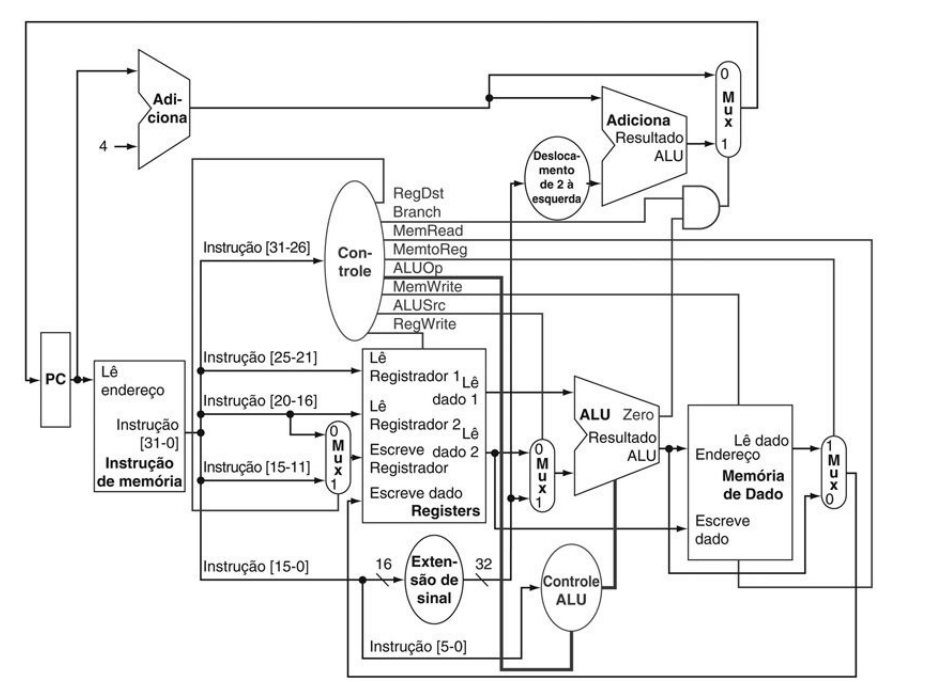
\includegraphics[width=\linewidth]{processadorRiscV.png}
\caption{O caminho de dados simples com a unidade de controle descrito no livro de Patterson e Hennessy (2017).}
\label{fig1}
\end{figure}

O RISC-V é uma ISA (Instruction Set Architecture) universal de tipo RISC (Reduced Instruction Set Computing) cuja principal característica é a modularidade. O RISC-V possui instruções básicas capazes de executar uma pilha completa de software de forma independente. Dizer que um processador RISC-V possui um pipeline de cinco estágios significa, portanto, que ele: (1) segue um ISA atômico e modular; (2) utiliza uma técnica de paralelismo em seu caminho de dados que permite que a execução de até cinco instruções se sobreponha simultaneamente no tempo para aumentar o rendimento e melhorar o desempenho. \citep{patterson2017riscv}

Dessa forma, neste trabalho adicionaremos funcionalidades ao pipeline para branch e controle de fluxo e hazard detection e forwarding, bem como executar um programa de teste para detecção de dependências e correção.

\section{Desenvolvimento}

\subsection{Branch e Controle de Fluxo}

O controle de fluxo pode ser definido como os mecanismos de instruções de saltos e desvios, que alteram a ordem de execução sequencial de um programa. Nesse contexto, um branch é uma instrução de desvio condicional que faz o processador saltar para o endereço de destino apenas se a comparação entre dois registradores for verdadeira. Caso a condição imposta não seja atendida, o processador executa a próxima instrução sequencial. \cite{patterson2017riscv}

Nesta etapa, implementamos o desvio condicional e tratamos hazards de controle.Para isso, implementamos: a instrução BEQ, a comparação de  operandos no estágio EX, o cálculo endereço de destino do branch e a atualização correta do Program Counter (PC).

Dessa forma, quando um branch é tomado, o PC passa a apontar para o endereço correto e as instruções já carregadas são descartadas.

\subsection{Execução do Programa de Teste}

Até este ponto, o caminho de dados do RISC-V ainda não possui mecanismos para a detecção de dependências e correção. O programa de teste em questão possui dependências e, portanto, sua execução não será bem sucedida. 

Nesta etapa, modificamos o código assembly para que o programa execute sem erros. Foi necessário reordenar instruções e adicionar nops no código do programa, bem como corrigir a label da instrução beq.

\subsection{Hazard Detection e Forwarding}

Por fim, implementamos a lógica de controle de hazards no
pipeline. A seleção dos operandos da Unidade Lógica Aritmética (ALU) foi feita, considerando forwarding dos estágio MEM, WB (ALU) e WB (load), bem como a detecção de hazards do tipo load-use, inserindo stall quando necessário.

\section{Resultados Obtidos}

\section{Conclusão}

\section*{Declarações}

\subsection*{Disponibilidade do Material}

O código-fonte deste relatório está disponível publicamente em https://github.com/davipuddo/Arq3-TP2.

\subsection*{Uso de IA}

Não foi utilizado nenhum conteúdo gerado por inteligência artificial na confecção do código ou na redação deste relatório.

\bibliographystyle{apalike-sol}
\bibliography{refs}

\end{document}
